\chapter{Phát triển dịch vụ phát hiện mã độc trên máy endpoint và dịch vụ phân tích mã độc online}

\section{Phân tích yêu cầu hệ thống}

\subsection{Yêu cầu chức năng}

Hệ thống được thiết kế để cung cấp hai lớp bảo vệ bổ sung cho nhau:
lớp phát hiện nhanh tại endpoint và lớp phân tích chuyên sâu trực
tuyến (online).

\textbf{Tại máy endpoint}, hệ thống cần đáp ứng các yêu cầu chức năng
sau:
\begin{itemize}
    \item Tự động phát hiện và chặn thực thi file PE bị phân loại là
        mã độc ngay tại thời điểm tiến trình được tạo, mà không yêu
        cầu thao tác thủ công từ người dùng.
    \item Hiển thị thông báo (popup) ngay lập tức khi phát hiện và
        chặn một mã độc mới.
    \item Cho phép người dùng xem lịch sử các lần phát hiện, bao gồm
        đường dẫn file và điểm đánh giá mức độ nguy hiểm
        (severity score).
    \item Cho phép người dùng submit file đáng ngờ lên dịch vụ phân
        tích sâu trực tuyến để nhận kết quả chi tiết hơn.
\end{itemize}

\textbf{Tại dịch vụ phân tích sâu trực tuyến
(deep-analysis-server)}, hệ thống cần đáp ứng các yêu cầu sau:
\begin{itemize}
    \item Nhận file PE từ người dùng thông qua giao diện web hoặc
        REST API.
    \item Thực hiện phân tích đầy đủ theo pipeline c (EMBER2024 +
        Capa + TruncatedSVD-256 + LightGBM + SHAP) và trả về kết quả
        phân loại cùng giải thích chi tiết.
    \item Hiển thị danh sách từng đặc trưng và mức độ đóng góp
        (contribution) vào quyết định phân loại, sắp xếp theo thứ tự
        giảm dần; đồng thời tổng hợp theo nhóm đặc trưng.
    \item Lưu trữ kết quả phân tích theo hash của file, tránh phân
        tích lại các file đã từng được xử lý thành công.
    \item Cung cấp chức năng thử lại (Retry) đối với các file đã
        upload nhưng quá trình phân tích gặp lỗi ngoại lệ (exception), mà không
        yêu cầu người dùng upload lại file.
\end{itemize}




\subsection{Yêu cầu phi chức năng}

\begin{itemize}
    \item \textbf{Hiệu năng tại endpoint:} Quá trình trích xuất đặc
        trưng và suy luận mô hình cần hoàn thành trong thời gian đủ
        ngắn để không gây trải nghiệm chờ đợi đáng chú ý cho người
        dùng. Đây là lý do module trích xuất đặc trưng được cài đặt
        bằng C++ thay vì Python (xem Mục~\ref{sec:fe_cpp}).
    \item \textbf{Quyền hệ thống:} pmd-service và pmd-ui cần được
        chạy với quyền quản trị (administrator) để có thể giao tiếp
        với driver qua IOCTL. pmd-service tự cài đặt vào danh mục
        Windows service và được cấu hình khởi động cùng hệ điều hành.
    \item \textbf{Hạn chế triển khai driver:} Driver trong phạm vi đề tài
    không được ký bằng chứng thực số (codesigning) cho môi
    trường production, do đó việc nạp driver chỉ được thực hiện trên
    máy ảo thử nghiệm đã được provisioning phục vụ phát triển driver
    (thông qua WDK/Visual Studio, sử dụng tài khoản WDKRemoteUser và
    cơ chế test signing).

    Nguyên nhân là trên các phiên bản Windows 10/11 64-bit hiện đại,
    đặc biệt khi Secure Boot được bật, kernel-mode driver thường phải
    được Microsoft xác thực chữ ký thông qua Hardware Dev Center.
    Quy trình này yêu cầu nhà phát triển sở hữu tài khoản Microsoft
    Partner Center đã được xác minh cùng chứng thư số Extended
    Validation (EV Code Signing Certificate) do tổ chức chứng thực
    (Certificate Authority) được Microsoft tin cậy cấp phát. Các yêu
    cầu này phát sinh chi phí đáng kể và nằm ngoài phạm vi của đề tài.

    Hạn chế trên được chấp nhận do mục tiêu chính của hệ thống là
    nghiên cứu kiến trúc và kiểm chứng tính khả thi của giải pháp,
    thay vì triển khai trên môi trường thực tế với người dùng thật.

    \item \textbf{Tính sẵn sàng của dịch vụ online:} Deep-analysis-server
        được đóng gói bằng Docker, đảm bảo tính nhất quán về môi
        trường thực thi và đơn giản hóa quá trình triển khai.
\end{itemize}

\subsection{Tổng quan các thành phần hệ thống}

Hệ thống gồm năm thành phần chính, được mô tả tổng quan trong
Bảng~\ref{tab:modules} và Hình~\ref{fig:system_arch}.

\begin{table}[h]
\centering
\caption{Các thành phần chính của hệ thống}
\label{tab:modules}
\begin{tabular}{llp{7cm}}
\toprule
\textbf{Module} & \textbf{Ngôn ngữ} & \textbf{Chức năng chính} \\
\midrule
ember2024-fe-cpp & C++, CMake   & Trích xuất vector đặc trưng EMBERv3
                                  từ file PE \\
pmd-driver       & C, KMDF      & Phát hiện tiến trình mới, giao tiếp
                                  với pmd-service qua IOCTL \\
pmd-service      & C++          & Windows service nhận scan task, chạy
                                  mô hình ML, trả verdict \\
pmd-ui           & C++, Win API & Hiển thị lịch sử phát hiện, thông
                                  báo mã độc, submit file online \\
deep-analysis-server & Python, FastAPI & Phân tích sâu với Capa +
                                  SVD-256 + SHAP, giao diện web \\
\bottomrule
\end{tabular}
\end{table}

\begin{figure}[h]
    \centering
    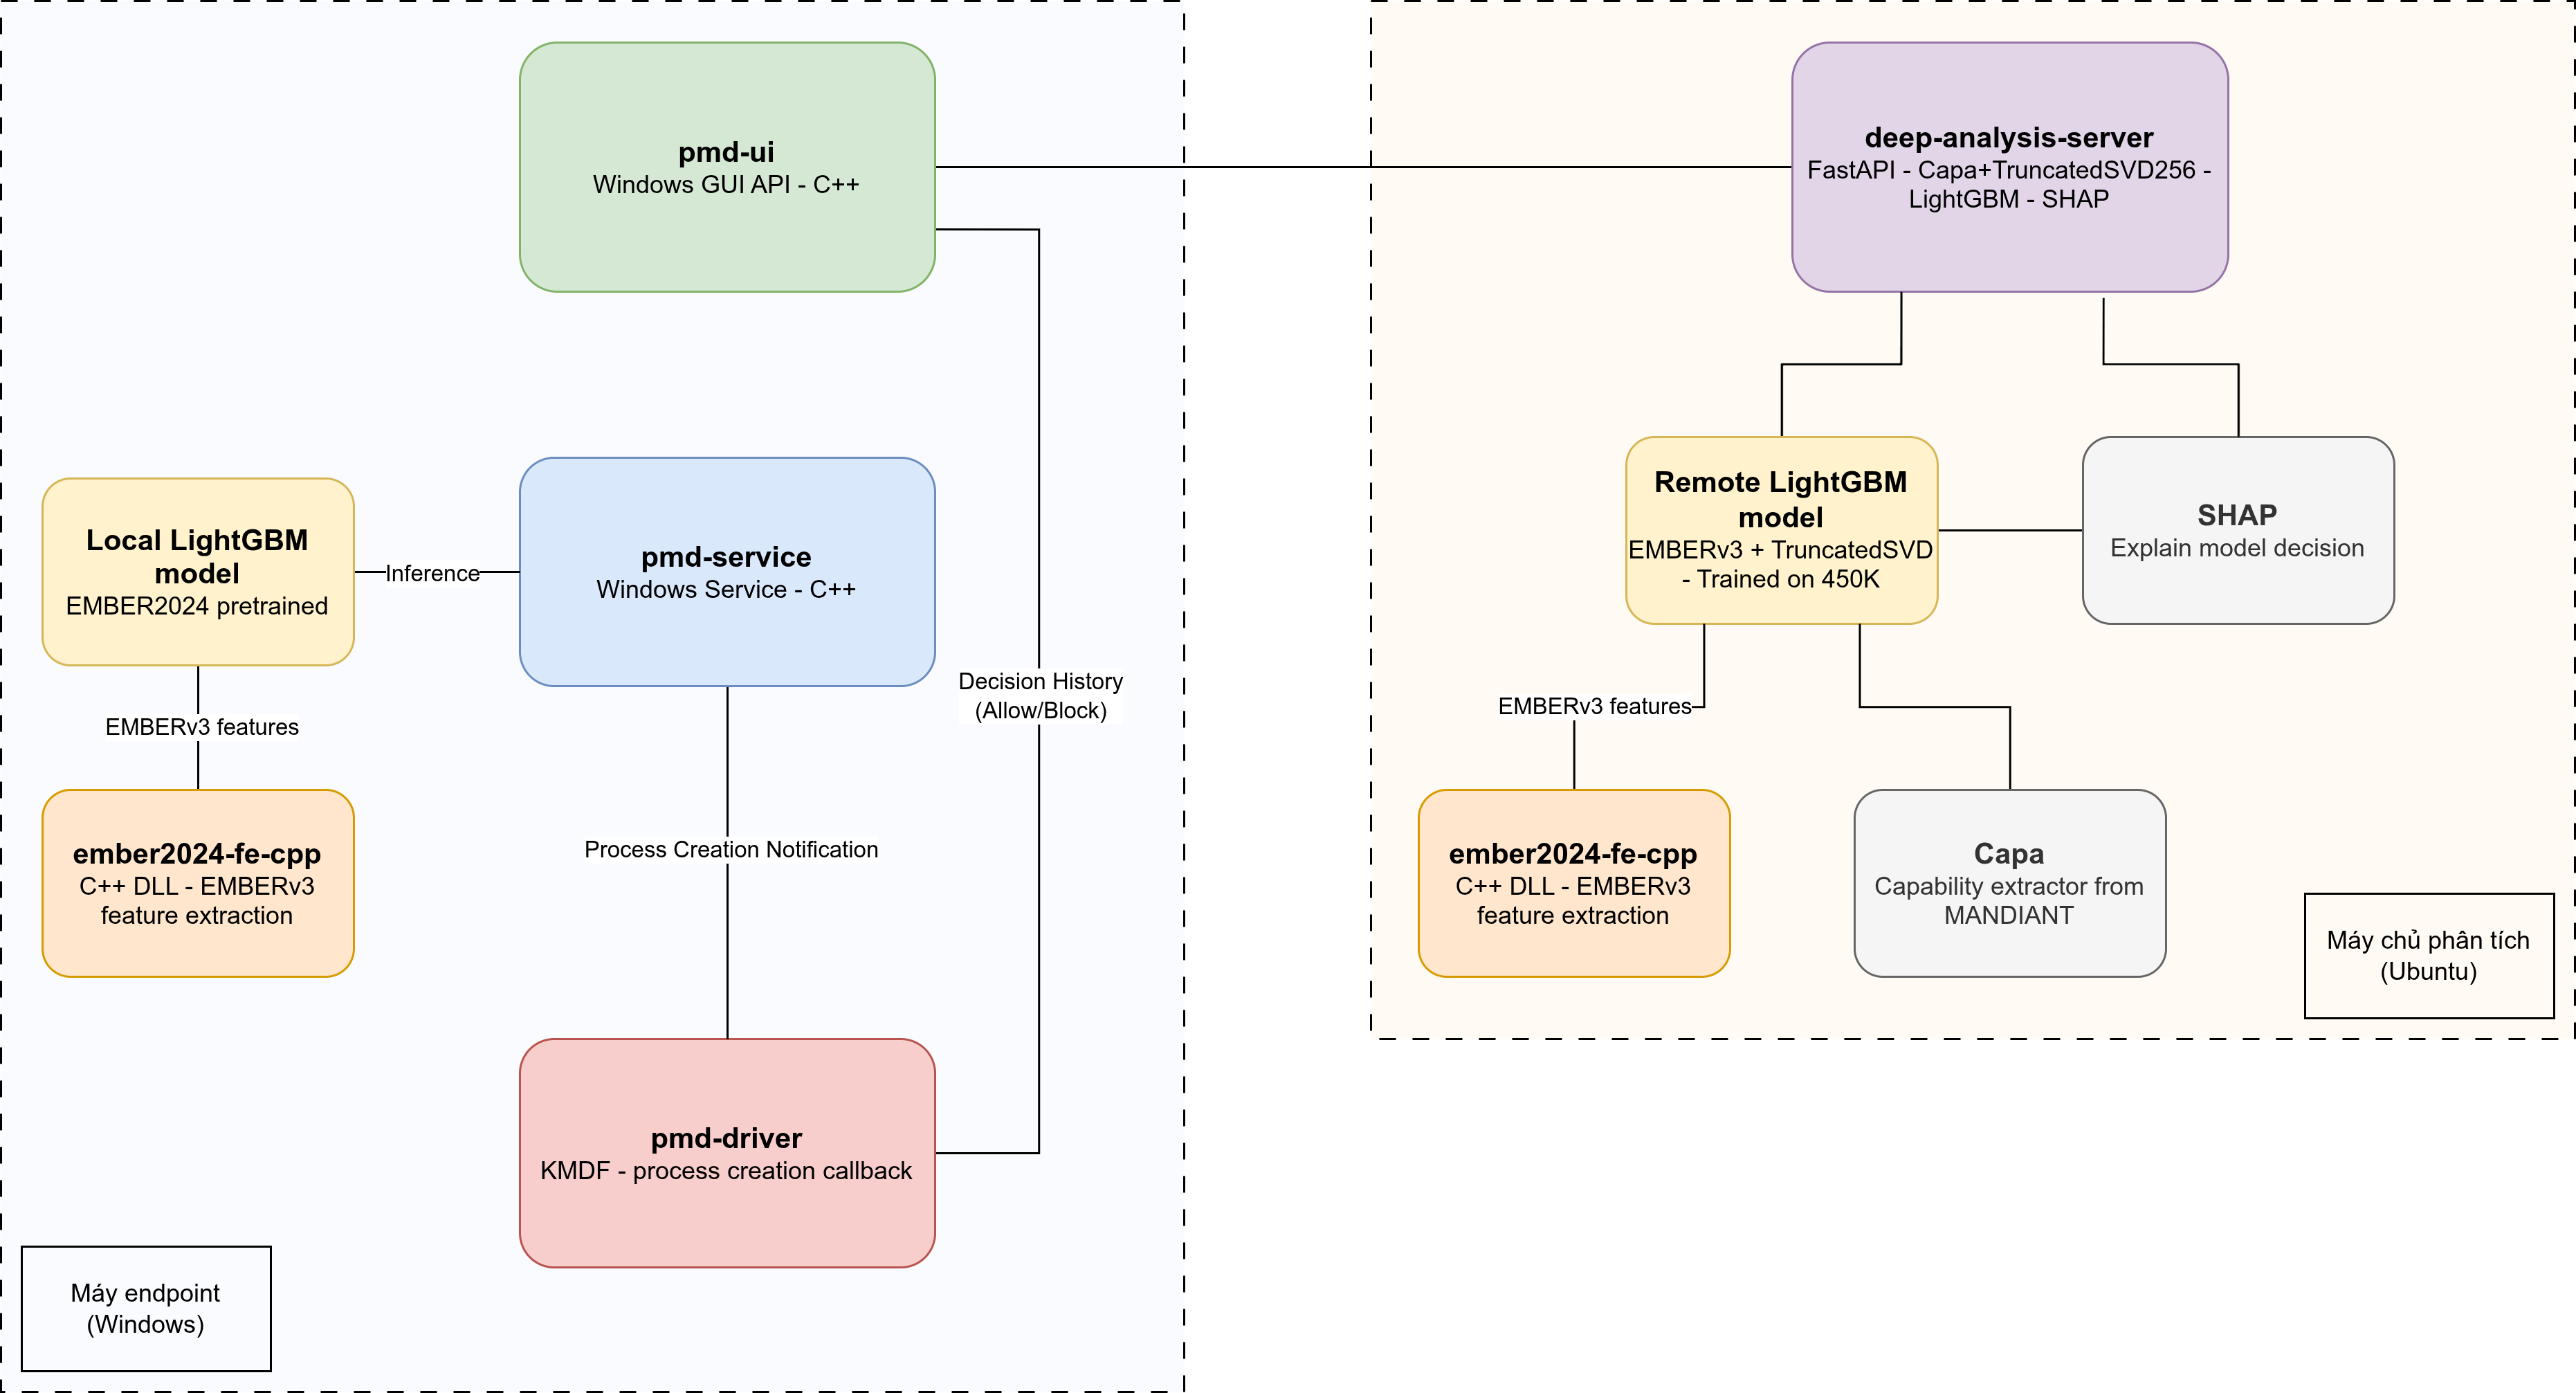
\includegraphics[width=\textwidth]{figures/system-diagram.png}
    \caption{Kiến trúc tổng thể của hệ thống phát hiện mã độc trên
    máy endpoint.}
    \label{fig:system_arch}
\end{figure}

\begin{figure}[h]
    \centering
    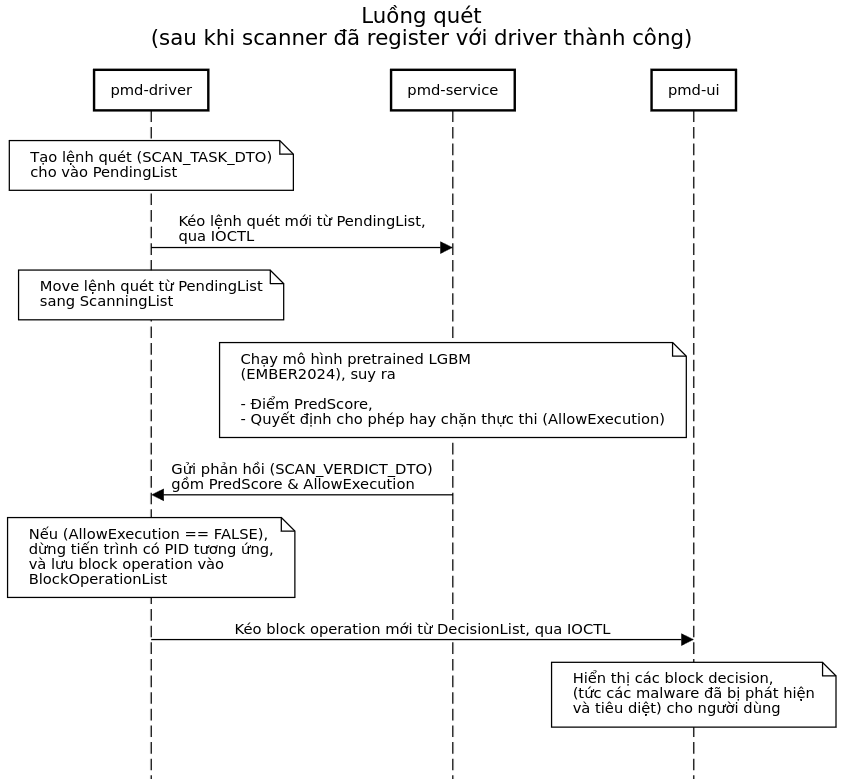
\includegraphics[width=\textwidth]{figures/endpoint-sequence-diagram.png}
    \caption{Sequence diagram thể hiện luồng quét file PE tại máy endpoint}
    \label{fig:endpoint_sequence_diagram}
\end{figure}

















\section{Thiết kế hệ thống chi tiết}

\subsection{Module trích xuất đặc trưng (ember2024-fe-cpp)}
\label{sec:fe_cpp}

Module ember2024-fe-cpp cài đặt lại pipeline trích xuất đặc trưng
EMBERv3 bằng C++, cho phép tích hợp trực tiếp vào các thành phần
hệ thống mà không cần phụ thuộc vào môi trường Python. Module được
quản lý bằng CMake và được biên dịch (compile) thành một thư viện
liên kết động (DLL) để có thể được sử dụng bởi pmd-service (qua
lời gọi hàm LoadLibrary) và deep-analysis-server (qua Python FFI).

Lý do cốt lõi cho quyết định cài đặt lại bằng C++ là yêu cầu hiệu
năng tại endpoint: trích xuất đặc trưng cần hoàn thành trong thời
gian đủ ngắn để không block tiến trình đang chờ kết quả quét từ pmd-service.
Bảng~\ref{tab:fe_perf} trình bày kết quả so sánh hiệu năng giữa cài
đặt Python gốc và cài đặt C++ trên các file PE có kích thước khác
nhau.

\begin{table}[h]
\centering
\caption{So sánh hiệu năng giữa hai bộ trích xuất đặc trưng EMBER2024
- Python và C++}
\label{tab:fe_perf}
\begin{tabular}{cccc}
\toprule
\textbf{Kích thước file PE} &
\textbf{Python (giây)} &
\textbf{C++ (giây)} &
\textbf{Tăng tốc} \\
\midrule
1,5 MB  & 0,657  & 0,053 & 1240\% \\
4,5 MB  & 1,519  & 0,114 & 1332\% \\
28,7 MB & 13,904 & 0,689 & 2018\% \\
\bottomrule
\end{tabular}
\end{table}

Kết quả cho thấy cài đặt C++ nhanh hơn cài đặt Python từ 12 đến
20 lần tùy theo kích thước file, với mức tăng tốc càng lớn khi file
càng lớn. Điều này đặc biệt quan trọng với các file PE lớn - vốn
phổ biến trong các bộ cài đặt phần mềm - nơi cài đặt Python mất
gần 14 giây trong khi cài đặt C++ chỉ cần dưới 0.7 giây.

\subsection{Module driver (pmd-driver)}

pmd-driver được viết bằng C, dựa trên KMDF (Kernel-Mode Driver
Framework). Driver sử dụng cơ chế \textbf{process creation callback}
để nhận thông báo từ hệ điều hành mỗi khi có một tiến trình mới được
tạo, từ đó phát hiện các lần thực thi file PE.

\textbf{Cơ chế hoạt động.}
Khi được nạp vào hệ điều hành, driver ở trạng thái nghỉ và chưa theo
dõi bất kỳ tiến trình nào. Trạng thái này kéo dài cho đến khi
pmd-service gửi một IOCTL đặc biệt để đăng ký (register), thông báo
cho driver rằng đã có một scanner sẵn sàng nhận và xử lý các yêu cầu
quét. Sau khi đăng ký thành công, mỗi khi phát hiện một tiến trình
mới, driver tạo một lệnh quét (scan task) dưới dạng
\texttt{SCAN\_TASK\_DTO} với các trường thông tin sau:
\begin{itemize}
    \item \texttt{PID}: định danh của tiến trình cần quét.
    \item \texttt{FileID} (128-bit): định danh duy nhất của file PE
        trên hệ thống file.
    \item \texttt{VolumeSerialNumber}: serial number của ổ đĩa chứa
        file PE.
    \item \texttt{Timestamp}: thời điểm tạo lệnh quét.
\end{itemize}

Lệnh quét được gửi lên pmd-service qua IOCTL. Driver sau đó chờ phản
hồi dưới dạng \texttt{SCAN\_VERDICT\_DTO} từ pmd-service, bao gồm:
\begin{itemize}
    \item \texttt{PID}, \texttt{FileID}, \texttt{VolumeSerialNumber}:
        định danh tiến trình và file đã quét.
    \item \texttt{PredScore}: xác suất file là mã độc (kiểu
        \texttt{double}, trong khoảng $[0.0,\ 1.0]$).
    \item \texttt{AllowExecution}: quyết định cho phép hay chặn thực
        thi (kiểu \texttt{BOOLEAN}).
\end{itemize}

Dựa trên \texttt{AllowExecution}, driver thực hiện một trong hai
hành động: nếu \texttt{TRUE}, tiến trình được phép chạy bình thường;
nếu \texttt{FALSE}, driver lập tức dừng (terminate) tiến trình có
\texttt{PID} tương ứng và lưu lại quyết định chặn dưới dạng struct
\texttt{BLOCK\_OPERATION\_DTO} để pmd-ui có thể đọc lịch sử.

\subsection{Module dịch vụ nền (pmd-service)}

pmd-service là một Windows service viết bằng C++, đóng vai trò là
bộ quét (scanner) trung tâm tại endpoint. Service cần được cài đặt
với flag \texttt{-install} dưới quyền administrator, sau đó được đăng
ký vào danh mục Windows service với cấu hình tự khởi động cùng hệ
điều hành.

\textbf{Quy trình khởi động và đăng ký với driver.}
Khi service khởi động, bước đầu tiên là gửi một IOCTL đăng ký đến
driver để thông báo rằng scanner đã sẵn sàng. Chỉ sau khi đăng ký
thành công, driver mới bắt đầu gửi các scan task xuống service.

\textbf{Luồng xử lý một scan task.}
Khi nhận được \texttt{SCAN\_TASK\_DTO} từ driver, pmd-service thực
hiện các bước sau:
\begin{enumerate}
    \item Định vị file PE trên hệ thống file dựa trên
        \texttt{FileID} và \texttt{VolumeSerialNumber}.
    \item Gọi ember2024-fe-cpp để trích xuất vector đặc trưng EMBERv3
        2.568 chiều từ file PE.
    \item Đưa vector đặc trưng vào mô hình LightGBM pretrained
        (EMBER2024) để nhận điểm \texttt{PredScore}.
    \item So sánh \texttt{PredScore} với ngưỡng phát hiện đã định
        trước để xác định \texttt{AllowExecution}.
    \item Gửi \texttt{SCAN\_VERDICT\_DTO} phản hồi về driver qua IOCTL.
\end{enumerate}

\subsection{Module giao diện người dùng (pmd-ui)}

pmd-ui là ứng dụng Windows với giao diện đồ họa (GUI) đơn giản, viết
bằng C++ và chỉ sử dụng Windows API. Ứng dụng cần được chạy với
quyền administrator để có thể giao tiếp với driver qua IOCTL.

pmd-ui cung cấp các chức năng sau:
\begin{itemize}
    \item \textbf{Hiển thị lịch sử phát hiện:} đọc danh sách các
        \texttt{BLOCK\_OPERATION\_DTO} từ driver, hiển thị thông tin
        từng lần chặn bao gồm đường dẫn file và điểm
        \texttt{PredScore}.
    \item \textbf{Thông báo thời gian thực:} hiển thị popup ngay khi
        driver phát hiện và chặn một mã độc mới.
    \item \textbf{Submit phân tích sâu:} từ màn hình chi tiết của một
        lần phát hiện, người dùng có thể submit file lên
        deep-analysis-server để nhận phân tích đầy đủ với giải thích
        SHAP.
\end{itemize}

\begin{figure}[h]
    \centering
    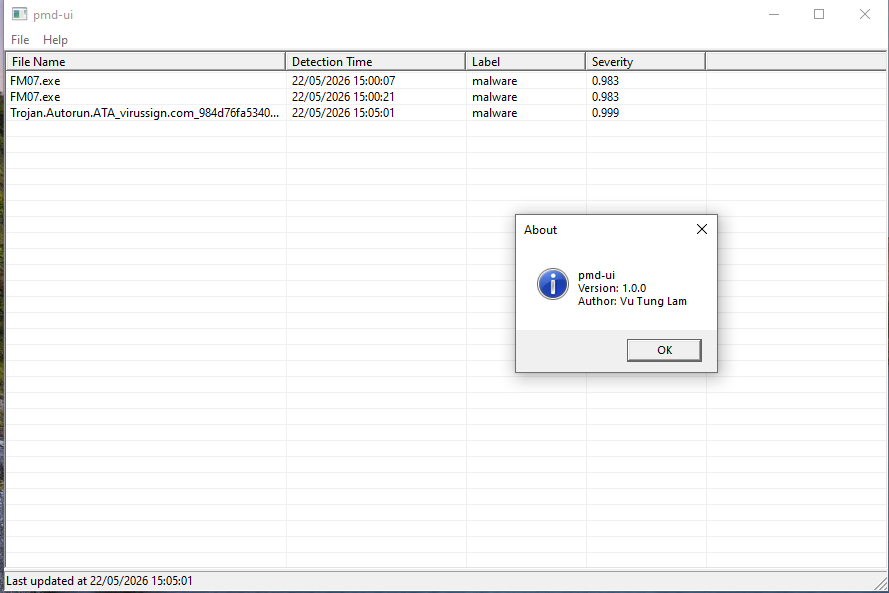
\includegraphics[width=\textwidth]{figures/pmd-ui.png}
    \caption{Giao diện chính của pmd-ui hiển thị lịch sử các lần
    phát hiện mã độc.}
    \label{fig:pmd_ui}
\end{figure}

\begin{figure}[h]
    \centering
    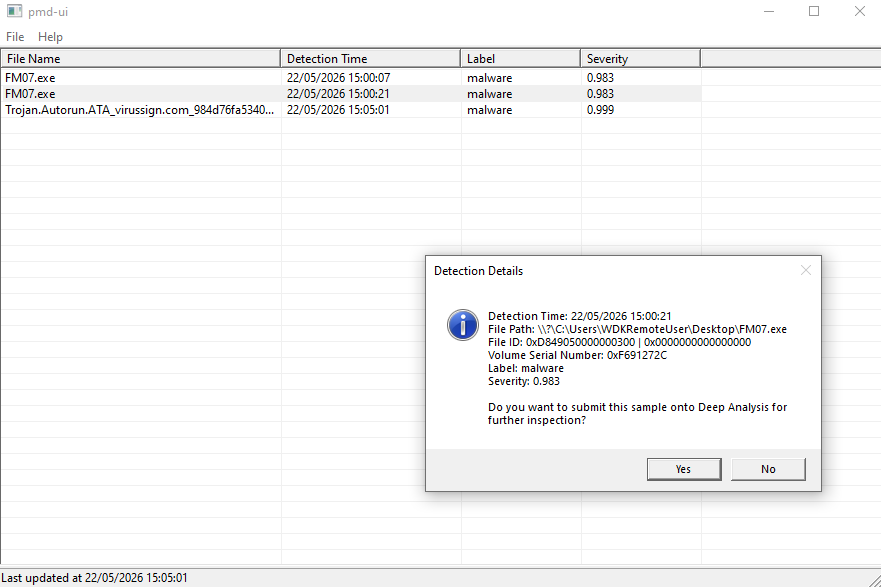
\includegraphics[width=\textwidth]{figures/pmd-ui-wanna-submit.png}
    \caption{Giao diện của pmd-ui gợi ý gửi mã độc lên dịch vụ phân tích chuyên sâu (deep-analysis-server).}
    \label{fig:pmd_ui_wanna_submit}
\end{figure}

\subsection{Module phân tích sâu (deep-analysis-server)}

deep-analysis-server là dịch vụ REST API viết bằng Python với
framework FastAPI, được đóng gói bằng Docker. Dịch vụ này triển khai
pipeline c (EMBER2024 + Capa + TruncatedSVD-256 + LightGBM + SHAP)
và cung cấp giao diện web để người dùng tương tác.

\textbf{Luồng xử lý phân tích.}
Khi nhận được một file PE (qua giao diện web hoặc API), dịch vụ
thực hiện các bước sau:
\begin{enumerate}
    \item Tính hash của file và kiểm tra cơ sở dữ liệu lưu trữ kết
        quả. Nếu file đã được phân tích thành công trước đó, trả về
        kết quả đã lưu mà không phân tích lại.
    \item Gọi ember2024-fe-cpp để trích xuất vector đặc trưng EMBERv3.
    \item Chạy Capa trên file PE để lấy danh sách capability, sau đó
        mã hóa one-hot và giảm chiều xuống 256 chiều bằng
        TruncatedSVD đã được huấn luyện từ trước.
    \item Ghép nối vector EMBER2024 và vector Capa đã giảm chiều,
        đưa vào mô hình LightGBM để nhận \texttt{PredScore} (xác suất
        file là mã độc - nhận giá trị từ 0.0 đến 1.0).
    \item Tính toán SHAP values cho kết quả dự đoán, tổng hợp theo
        từng đặc trưng và theo nhóm đặc trưng.
    \item Lưu kết quả vào cơ sở dữ liệu theo hash file.
\end{enumerate}

Nếu bất kỳ bước nào phát sinh ngoại lệ (exception), kết quả được lưu
với trạng thái lỗi. Người dùng có thể kích hoạt lại phân tích bằng
chức năng \textbf{Retry} mà không cần upload lại file (nếu quá
trình upload file đã thành công trước đó).

\textbf{Kết quả phân tích trả về} bao gồm:
\begin{itemize}
    \item Nhãn phân loại (lành tính / mã độc) và điểm
        \texttt{PredScore}.
    \item Danh sách từng đặc trưng và giá trị SHAP contribution tương
        ứng, sắp xếp theo thứ tự đóng góp giảm dần.
    \item Danh sách các nhóm đặc trưng (PE header, section, import
        table, chuỗi văn bản, nội dung nhị phân, Capa\dots) và tổng
        SHAP contribution của từng nhóm, sắp xếp theo thứ tự giảm
        dần.
\end{itemize}

\begin{figure}[h]
    \centering
    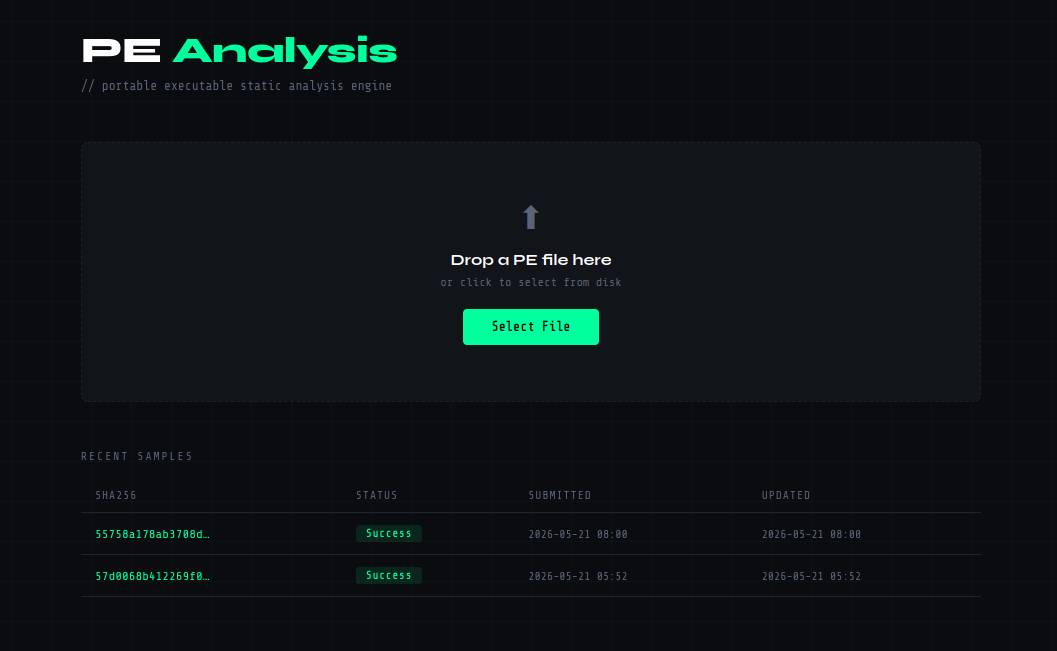
\includegraphics[width=\textwidth]{figures/deep-analysis-server-homepage.png}
    \caption{Giao diện web của deep-analysis-server, cho phép người dùng upload file thủ công.}
    \label{fig:deep_analysis}
\end{figure}

% ==================================================================
\section{Cài đặt và kiểm thử}
% ==================================================================

\subsection{Môi trường cài đặt}

\begin{table}[h]
\centering
\caption{Môi trường cài đặt và kiểm thử}
\label{tab:env}
\begin{tabular}{ll}
\toprule
\textbf{Thành phần} & \textbf{Cấu hình} \\
\midrule
% [Placeholder: bổ sung thông tin phần cứng, OS, phiên bản công cụ]
Hệ điều hành        & Windows 10 (đã tắt Windows Defender) \\
Máy ảo driver       & Windows (WDKRemoteUser, Provisioning mode) \\
Ngôn ngữ / Runtime  & C++ (MSVC 2022), Python 3.12, CMake \\
Framework driver    & KMDF (Windows Driver Kit) \\
Docker              & Docker Engine on Ubuntu 22.04 \\
\bottomrule
\end{tabular}
\end{table}

\subsection{Mô tả phần tự cài đặt và phần tận dụng}

Bảng~\ref{tab:impl} mô tả phân tách giữa phần sinh viên tự cài đặt
và phần tận dụng từ thư viện hoặc công cụ bên ngoài.

\begin{table}[h]
\centering
\caption{Phân tách phần tự cài đặt và phần tận dụng}
\label{tab:impl}

\begin{tabularx}{\textwidth}{|p{3cm}|p{2.5cm}|X|}
\hline

\textbf{Thành phần} &
\textbf{Loại} &
\textbf{Mô tả} \\
\hline

ember2024-fe-cpp &
Tự cài đặt &
Cài đặt lại pipeline EMBERv3 bằng C++ \\
\hline

pmd-driver &
Tự cài đặt &
KMDF driver với process creation callback, IOCTL \\
\hline

pmd-service &
Tự cài đặt &
Windows service, tích hợp ember2024-fe-cpp \\
\hline

pmd-ui &
Tự cài đặt &
GUI Windows API, đọc IOCTL, submit file online \\
\hline

FastAPI server &
Tự cài đặt &
REST API, luồng phân tích, lưu kết quả theo hash \\
\hline

Giao diện web &
Tự cài đặt &
HTML/CSS/JS, hiển thị SHAP, Retry \\
\hline

LightGBM (EMBER2024) &
Tận dụng &
Pretrained model do nhóm tác giả EMBER2024 cung cấp \\
\hline

Capa &
Tận dụng &
Công cụ capability extraction (Mandiant) \\
\hline

SHAP &
Tận dụng &
Thư viện giải thích mô hình (xAI) \\
\hline

TruncatedSVD &
Tận dụng &
scikit-learn, fit trên tập huấn luyện 450K mẫu \\
\hline

KMDF Framework &
Tận dụng &
Windows Driver Kit (Microsoft) \\
\hline

\end{tabularx}

\end{table}

\subsection{Kịch bản kiểm thử end-to-end}

Các kịch bản kiểm thử tập trung vào luồng hoạt động tổng thể của hệ
thống, từ thời điểm file PE được thực thi đến khi người dùng nhận
được kết quả phân tích.

\begin{table}[h]
\centering
\caption{Kịch bản kiểm thử end-to-end}
\label{tab:testcases}
\begin{tabular}{clp{4.5cm}p{4cm}}
\toprule
\textbf{TC} & \textbf{Mô tả} & \textbf{Đầu vào} &
\textbf{Kết quả kỳ vọng} \\
\midrule
TC1 & Thực thi file lành tính &
    File PE đã biết là lành tính &
    Tiến trình được phép chạy, không có thông báo \\
\midrule
TC2 & Thực thi file mã độc &
    File PE mã độc đã biết &
    Tiến trình bị terminate, popup thông báo xuất hiện trên pmd-ui \\
\midrule
TC3 & Xem chi tiết lần phát hiện &
    Chọn một mục trong lịch sử phát hiện &
    Hiển thị đường dẫn file và severity score \\
\midrule
TC4 & Submit phân tích sâu &
    Submit file từ TC2 lên deep-analysis-server &
    Nhận kết quả phân loại, danh sách feature contribution và nhóm
    feature contribution \\
\midrule
TC5 & Phân tích file đã biết &
    Upload lại file đã phân tích ở TC4 &
    Trả về kết quả đã lưu, không phân tích lại \\
\midrule
TC6 & Retry sau lỗi &
    Kích hoạt Retry trên file có trạng thái lỗi &
    Hệ thống phân tích lại mà không yêu cầu upload lại file \\
\bottomrule
\end{tabular}
\end{table}

\subsection{Kết quả kiểm thử và đánh giá hiệu năng}

\textbf{Kết quả kiểm thử.}

\begin{table}[h]
\centering
\caption{Kết quả kiểm thử end-to-end}
\label{tab:test_results}

\begin{tabularx}{\textwidth}{|c|X|c|X|}
\hline
\textbf{TC} &
\textbf{Mô tả} &
\textbf{Kết quả} &
\textbf{Ghi chú} \\
\hline

TC1 & Thực thi file lành tính &
Pass &
Hoạt động đúng như mong đợi \\

\hline

TC2 & Thực thi file mã độc &
Pass &
Phát hiện và cảnh báo thành công \\

\hline

TC3 & Xem chi tiết phát hiện &
Pass &
Hiển thị đầy đủ thông tin \\

\hline

TC4 & Submit phân tích sâu &
Pass &
Tác vụ được gửi thành công \\

\hline

TC5 & Phân tích file đã biết &
Pass &
Trả về kết quả từ cache \\

\hline

TC6 & Retry sau lỗi &
Pass &
Cho phép thực hiện lại tác vụ \\

\hline
\end{tabularx}

\end{table}

\begin{figure}[h]
    \centering
    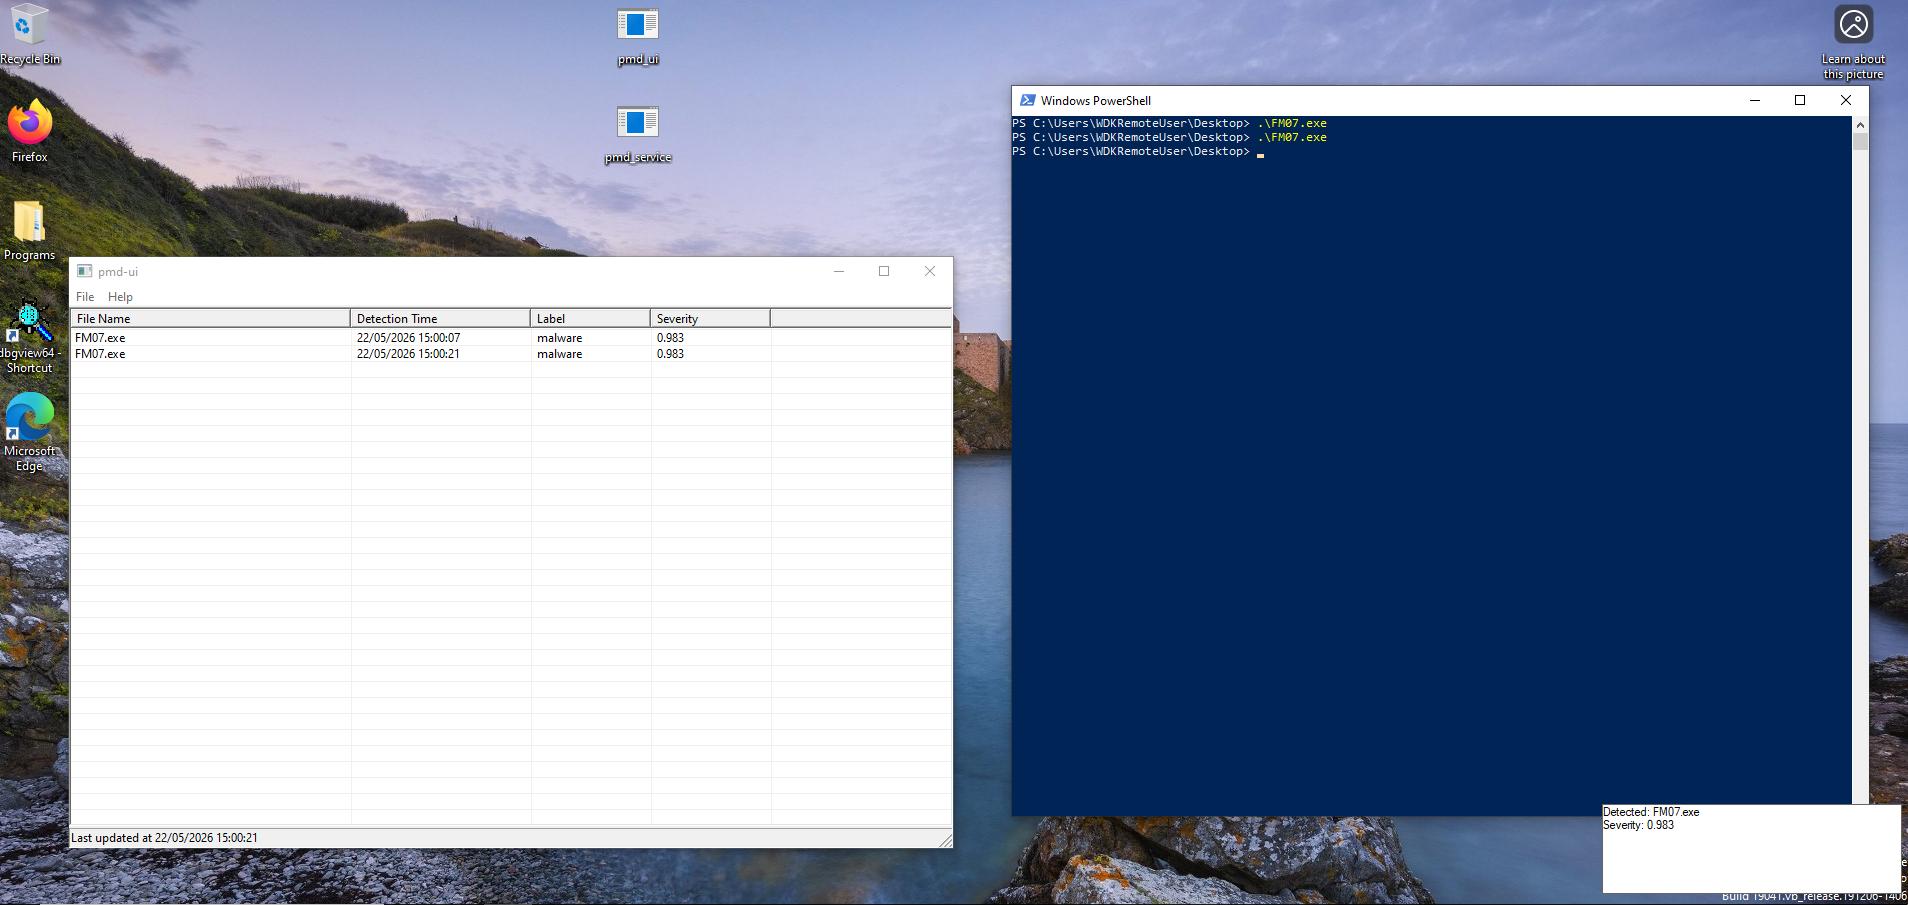
\includegraphics[width=\textwidth]{figures/tc2_block.png}
    \caption{Kết quả TC2: tiến trình bị terminate và popup thông báo
    trên pmd-ui.}
    \label{fig:tc2}
\end{figure}

\begin{figure}[h]
    \centering
    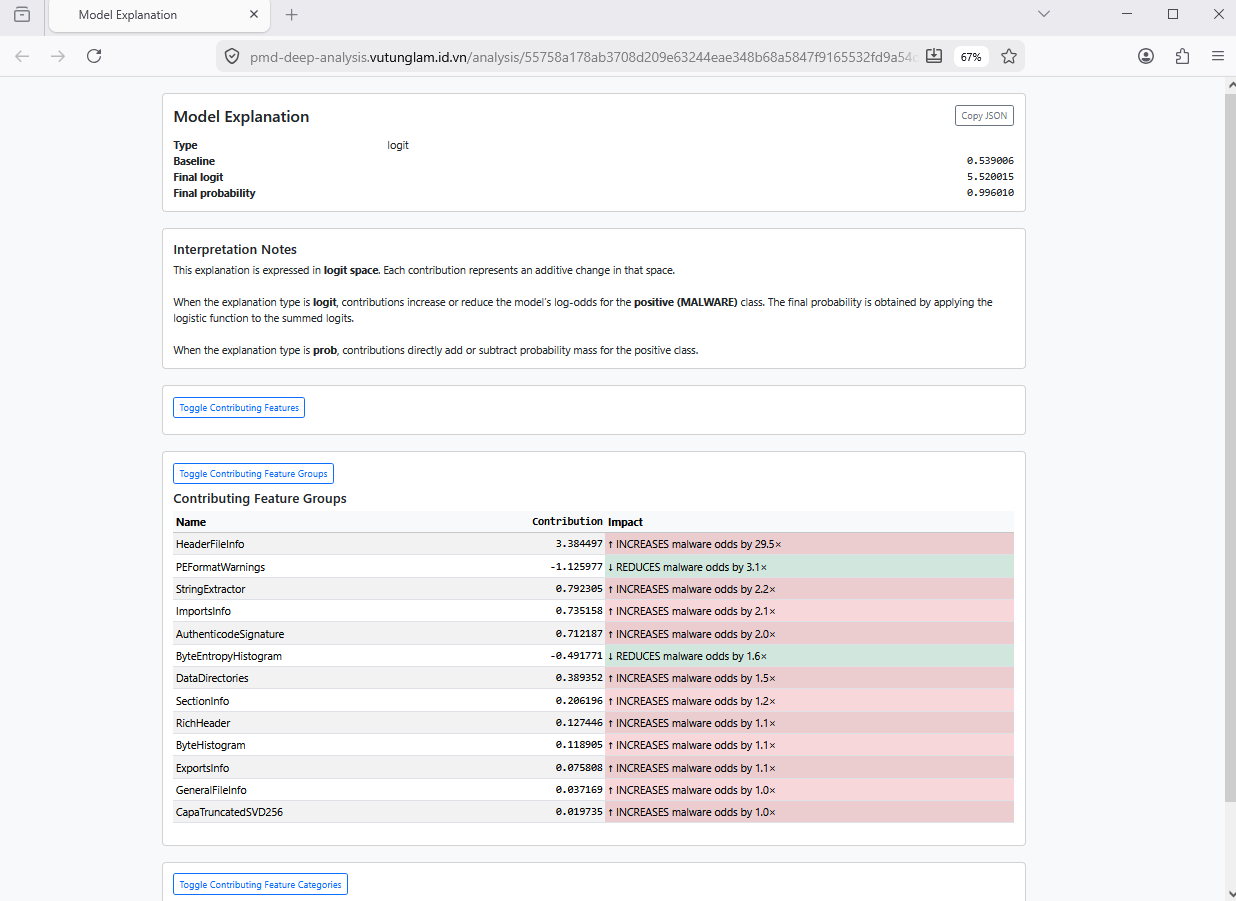
\includegraphics[width=\textwidth]{figures/tc4_shap.png}
    \caption{Kết quả TC4: giao diện deep-analysis-server hiển thị
    kết quả phân loại và danh sách đóng góp đặc trưng.}
    \label{fig:tc4}
\end{figure}

\textbf{Đánh giá hiệu năng trích xuất đặc trưng.}
Bảng~\ref{tab:fe_perf} (Mục~\ref{sec:fe_cpp}) đã trình bày kết quả
so sánh hiệu năng giữa cài đặt Python và C++ của bộ trích xuất đặc
trưng EMBER2024. Với mức tăng tốc từ 12 đến 20 lần, cài đặt C++ đảm
bảo rằng tổng thời gian xử lý tại endpoint - bao gồm trích xuất
đặc trưng và suy luận LightGBM - nằm trong giới hạn chấp nhận được
đối với người dùng cuối, kể cả với các file PE có kích thước lớn.
